\documentclass[a4paper,11pt]{article}

\usepackage[utf8]{inputenc} \usepackage[T1]{fontenc}
\usepackage{fancyhdr} \usepackage{graphicx,subfig} \usepackage{lastpage}
\usepackage{amssymb,amsmath} \usepackage{siunitx} \usepackage[nodayofweek]{datetime}
\usepackage[top=3.5cm,bottom=2.5cm,left=3cm,right=3cm,headheight=40pt]{geometry}
\usepackage{parskip} \usepackage{float} \usepackage{enumitem} \pagestyle{fancy}
\usepackage[colorlinks=true,allcolors=blue]{hyperref} \hypersetup{
	pdfauthor={Michaël Defferrard},
	pdftitle={Project stage 2: Rendering},
	pdfsubject={Introduction to Computer Graphics}
}

\lhead{Introduction to Computer Graphics\\Project stage 2: Rendering\\Group 19}
\chead{\hspace{2.5cm}EPFL\\\hspace{2.5cm}\shortdate\today\\\hspace{2.5cm}\thepage/\pageref{LastPage}}
\rhead{Michaël \textsc{Defferrard}\\Pierre \textsc{Fechting}\\Vu Hiep \textsc{Doan}}
\cfoot{}

\begin{document}


\section{Overview}

This report presents our advancement on the second part of the project : rendering using procedural methods. Figure~ shows an example of what our actual code base is able to generate. All the minimal steps to display a procedurally generated terrain were successfully completed. We did also implement some other optional suggested methods, like 


\section{Implementation}

\subsection{Improvement on the last stage}

\subsubsection{Parameter tuning for better terrain generation}

\subsubsection{Fixing normal vector calculation}
The normal vector calculation implemented in previous stage is actually not correct but only until we try to blend the texture based on the normal vector that we recognize that the results are not correct. While it costs us a lot of time to re-implement normal vector calculation, the experience that we learned when correcting the normal vector is really invaluable for further understanding OpenGL pipeline.

Firstly, we map the world coordinate to a texel before using \texttt{textureOffset} function to look up the height of surrounding texels in both x and y direction. A finite difference is used to approximate the tangent vector to the surface at that point on the height map then finally, a normal vector will be just the cross product of tangent vectors along x and y directions.

In addition, the above normal vector is just in height map coordinate (ranging from $[0,1] \times [0,1]$ in xy plane) so we need to map it to our world coordinate of the grid ([-1,1] in xy plane). Note that when transform the normal vector, we actually need to multiply it with the inverse of transpose matrix of the transformed one.

To test the normal vector, we output it as the color of each fragment as shown in Figure~\ref{normal_vector}. We can see that the result is quite reasonable, for example in the ground part as it is flat region, the normal vector should be (0,0,1) and as a result, its color is blue.


\begin{figure}[ht]
	\centering
	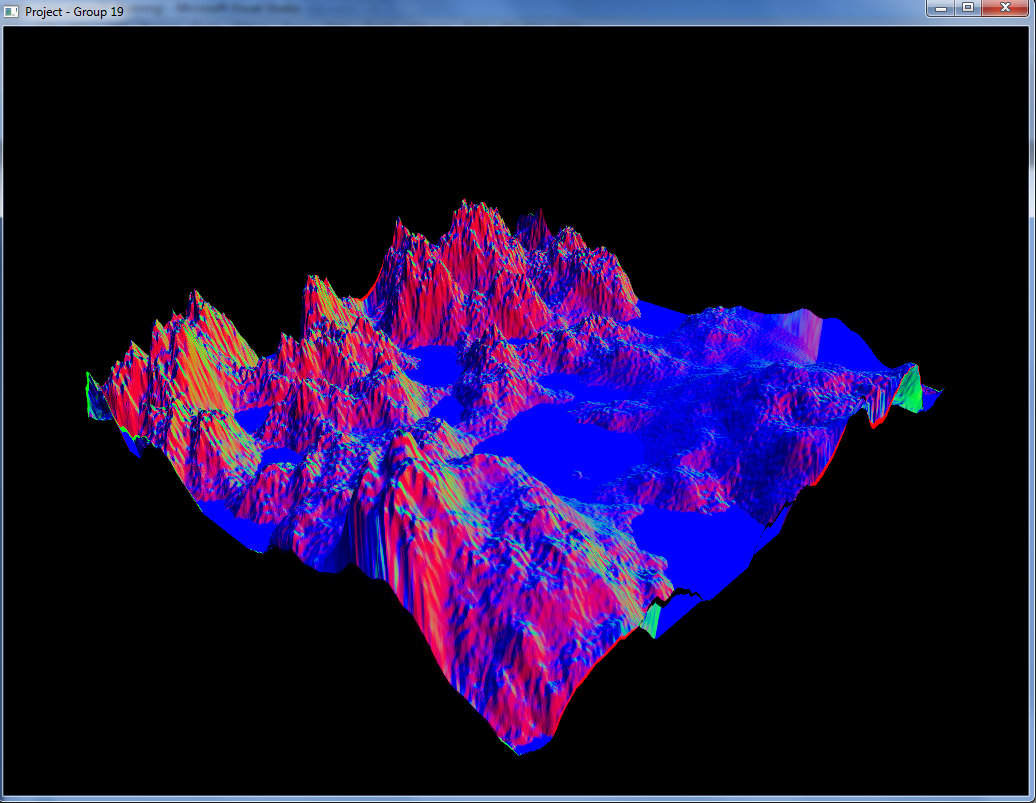
\includegraphics[height=4cm]{{{img_stage2/normal_vector}}}
	\caption{The terrain is colored by its own normal vector.}
	\label{normal_vector}
\end{figure}
\subsection{Basic}
\subsubsection{Texturing}
In this part, our idea is that we can use whatever texture that we want, whatever method or way of blending that we want as long as the terrain looks realistic. Also, the way we implement texture blending is trial and errors, we try many different ways of blending and continue in the direction that generates better results.


\begin{figure}[ht]
	\centering
	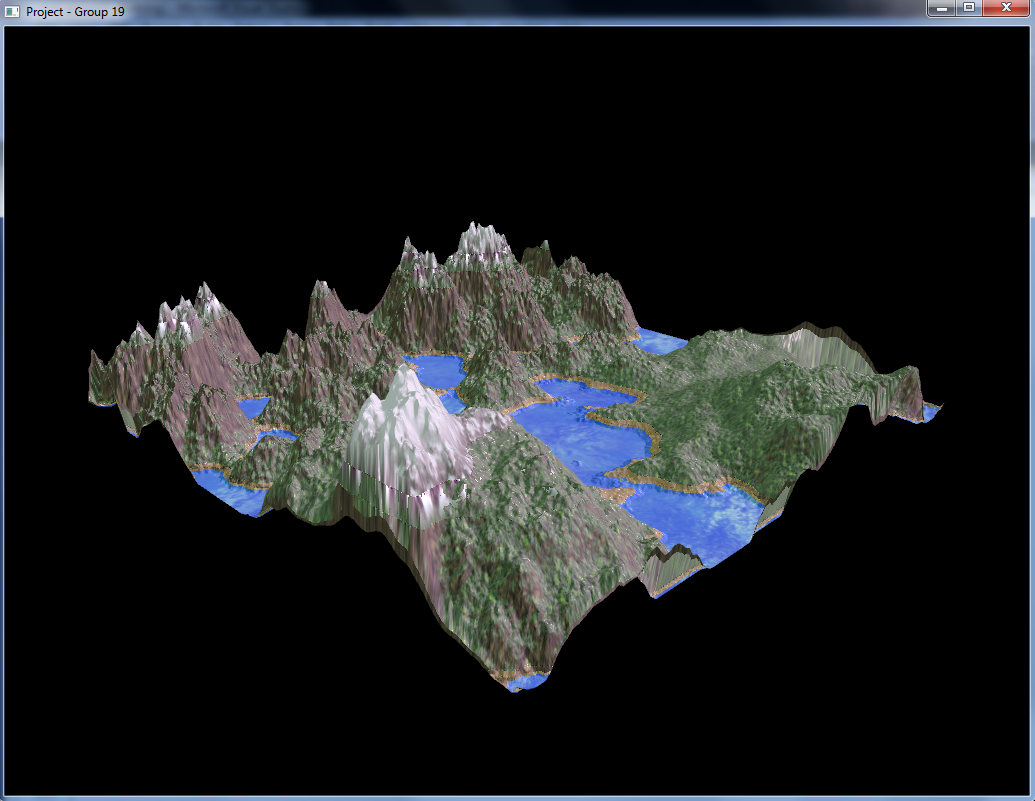
\includegraphics[height=4cm]{{{img_stage2/texture_blending_with_specular}}}
	\caption{The terrain with blended texture.}
	\label{texture_blending}
\end{figure}
\subsubsection{Modeling the sky}

\subsubsection{Self shadowing}


\subsection{Advanced}

\subsubsection{Approximating water reflections/refractions}

\subsubsection{Water depth effect (participating media)}

\subsubsection{Water dynamics}

\subsubsection{Time of the day}


\section{Results}


\end{document}
